\documentclass[12pt]{report}
\usepackage[utf8]{inputenc}
\usepackage[russian]{babel}
%\usepackage[14pt]{extsizes}
\usepackage{listings}
\usepackage{graphicx}
\usepackage{amsmath,amsfonts,amssymb,amsthm,mathtools} 
\usepackage{pgfplots}
\usepackage{filecontents}
\usepackage{indentfirst}
\usepackage{eucal}
\usepackage{enumitem}
\frenchspacing

\usepackage{indentfirst} % Красная строка


\usetikzlibrary{datavisualization}
\usetikzlibrary{datavisualization.formats.functions}

\usepackage{amsmath}




% Для листинга кода:
\lstset{ %
language=python,                 % выбор языка для подсветки
basicstyle=\small\sffamily, % размер и начертание шрифта для подсветки кода
numbers=left,               % где поставить нумерацию строк (слева\справа)
numberstyle=\tiny,           % размер шрифта для номеров строк
stepnumber=1,                   % размер шага между двумя номерами строк
numbersep=5pt,                % как далеко отстоят номера строк от подсвечиваемого кода
showspaces=false,            % показывать или нет пробелы специальными отступами
showstringspaces=false,      % показывать или нет пробелы в строках
showtabs=false,             % показывать или нет табуляцию в строках
frame=single,              % рисовать рамку вокруг кода
tabsize=2,                 % размер табуляции по умолчанию равен 2 пробелам
captionpos=t,              % позиция заголовка вверху [t] или внизу [b] 
breaklines=true,           % автоматически переносить строки (да\нет)
breakatwhitespace=false, % переносить строки только если есть пробел
escapeinside={\#*}{*)}   % если нужно добавить комментарии в коде
}

\usepackage[left=2cm,right=2cm, top=2cm,bottom=2cm,bindingoffset=0cm]{geometry}
% Для измененных титулов глав:
\usepackage{titlesec, blindtext, color} % подключаем нужные пакеты
\definecolor{gray75}{gray}{0.75} % определяем цвет
\newcommand{\hsp}{\hspace{20pt}} % длина линии в 20pt
% titleformat определяет стиль
\titleformat{\chapter}[hang]{\Huge\bfseries}{\thechapter\hsp\textcolor{gray75}{|}\hsp}{0pt}{\Huge\bfseries}


% plot
\usepackage{pgfplots}
\usepackage{filecontents}
\usetikzlibrary{datavisualization}
\usetikzlibrary{datavisualization.formats.functions}

\begin{document}
\thispagestyle{empty}
\begin{titlepage}
	\noindent \begin{minipage}{0.15\textwidth}
	
\includegraphics[width=\linewidth]{b_logo}
	\end{minipage}
	\noindent\begin{minipage}{0.9\textwidth}\centering
		\textbf{Министерство науки и высшего образования Российской Федерации}\\
		\textbf{Федеральное государственное бюджетное образовательное учреждение высшего образования}\\
		\textbf{~~~«Московский государственный технический университет имени Н.Э.~Баумана}\\
		\textbf{(национальный исследовательский университет)»}\\
		\textbf{(МГТУ им. Н.Э.~Баумана)}
	\end{minipage}
	
	\noindent\rule{18cm}{3pt}
	\newline\newline
	\noindent ФАКУЛЬТЕТ $\underline{\text{«Информатика и системы управления»}}$ \newline\newline
	\noindent КАФЕДРА $\underline{\text{«Программное обеспечение ЭВМ и информационные технологии»}}$\newline\newline\newline\newline\newline
	
	
	\begin{center}
		\noindent\begin{minipage}{1.3\textwidth}\centering
			\Large\textbf{  Отчет по лабораторной работе №7}\newline
			\textbf{по дисциплине "Анализ алгоритмов"}\newline\newline
		\end{minipage}
	\end{center}
	
	\noindent\textbf{Тема} $\underline{\text{Поиск в словаре}}$\newline\newline
	\noindent\textbf{Студент} $\underline{\text{Андрич К. }}$\newline\newline
	\noindent\textbf{Группа} $\underline{\text{ИУ7И-56Б}}$\newline\newline
	\noindent\textbf{Оценка (баллы)} $\underline{\text{~~~~~~~~~~~~~~~~~~~~~~~~~~~}}$\newline\newline
	\noindent\textbf{Преподаватели} $\underline{\text{Волкова Л.Л.}}$\newline\newline\newline
	
	\begin{center}
		\vfill
		Москва~---~\the\year
		~г.
	\end{center}
\end{titlepage}


\tableofcontents

\newpage
\chapter*{Введение}
\addcontentsline{toc}{chapter}{Введение}
Обычные списки (массивы) представляют собой набор пронумерованных элементов, то есть для обращения к какому-либо элементу списка необходимо указать его номер. Номер элемента в списке однозначно идентифицирует сам элемент. Но идентифицировать данные по числовым номерам не всегда оказывается удобно. 

Структура данных, позволяющая идентифицировать ее элементы не по числовому индексу, а по произвольному, называется словарем или ассоциативным массивом. Каждый элемент словаря состоит из двух объектов: ключа и значения. 
В жизни широко распространены словари, например, привычные бумажные словари (толковые, орфографические, лингвистические). В них ключом является слово-заголовок статьи, а значением — сама статья. Для того, чтобы получить доступ к статье, необходимо указать слово-ключ.

Другой пример словаря, как структуры данных — телефонный справочник. В нем ключом является имя, а значением — номер телефона. И словарь, и телефонный справочник хранятся так, что легко найти элемент словаря по известному ключу (например, если записи хранятся в алфавитном порядке ключей, то легко можно найти известный ключ, например, бинарным поиском), но если ключ неизвестен, а известно лишь значение, то поиск элемента с данным значением может потребовать последовательного просмотра всех элементов словаря.

Особенностью ассоциативного массива является его динамичность: в него можно добавлять новые элементы с произвольными ключами и удалять уже существующие элементы. При этом размер используемой памяти пропорционален размеру ассоциативного массива. Доступ к элементам ассоциативного массива выполняется хоть и медленнее, чем к обычным массивам, но в целом довольно быстро.

Словари нужно использовать в следующих случаях:
\begin{enumerate}
	\item Подсчет числа каких-то объектов. В этом случае нужно завести словарь, в котором ключами являются объекты, а значениями — их количество;
	\item Хранение каких-либо данных, связанных с объектом. Ключи — объекты, значения — связанные с ними данные;
	\item Установка соответствия между объектами (например, “родитель—потомок”). Ключ — объект, значение — соответствующий ему объект;
	\item Если нужен обычный массив, но при этом максимальное значение индекса элемента очень велико, но при этом будут использоваться не все возможные индексы (так называемый “разреженный массив”), то можно использовать ассоциативный массив для экономии памяти.
	
\end{enumerate}

\newpage

Цель данной лабораторной работы: изучить и реализовать алгоритмы поиска по словарю.

Для достижения поставленной цели требуется выполнить следующие задачи:
\begin{enumerate}
	\item Реализовать алгоритм поиска по словарю с использованием полного перебора, двоичного поиска, комбинированного алгоритма;
	
	\item Изучить алгоритм частотного анализа в задаче поиска по словарю;
	
	\item Провести тестирование работы алгоритмов в худшем, лучшем и произвольном случаях;
	
	\item Провести замеры процессорного времени работы алгоритмов поиска по словарю для каждого ключа и для отсутствующего ключа, вывести минимальное, максимальное и среднее время поиска ключа;
	
	\item Сделать выводы на основе произведённого исследования и описать в отчёте.
	
\end{enumerate}

\chapter{Аналитическая часть}

В данном разделе будет поставлена цель и описаны задачи, описаны алгоритмы которые будут использоваться в лабораторной работе.

\section{Алгоритм поиска в словаре с использованием полного перебора}

Все элементы словаря пересматриваются последовательно в порядке их размещения, пока не найдётся элемент, равный ключу поиска. Если не известно, есть ли искомый элемент, то необходимо следить, чтобы поиск не вышел за границы списка. В таком случае техничным способом повышения эффективности программирования является введение стопера.

\section{Алгоритм поиска в словре с использованием бинарного поиска}

Бинарный поиск производится в упорядоченном словаре.

При бинарном поиске искомый ключ сравнивается с ключом среднего элемента в словаре. Если они равны, то поиск успешен. В противном случае поиск осуществляется аналогично в левой или правой частях словаря.

Алгоритм может быть определен в рекурсивной и нерекурсивной формах.

Бинарный поиск также называют поиском методом деления отрезка пополам или дихотомии.

На каждом шаге осуществляется поиск середины отрезка по формуле $mid = (left + right) / 2$.

Если искомый элемент равен элементу с индексом mid, поиск завершается.
В случае если искомый элемент меньше элемента с индексом mid, на место mid перемещается правая граница рассматриваемого отрезка, в противном случае — левая граница.


\section{Комбинированный алгоритм}

Перед началом работы алгоритма поиска для словаря, полученного на вход, нужно произвести сегментацию по первой букве, затем выполнить частотный анализ. Для этого нужно для первой буквы каждого значения в словаре посчитать, сколько раз она встречается в качестве первой буквы у других значений. По полученным значениям словарь разбивается на сегменты так, что все элементы с одинаковой первой буквой оказались в одном сегменте. Сегменты сортируются по частоте первых букв. Далее каждый сегмент сортируется в лексикографическом порядке, чтобы можно было применить бинарный поиск в сегменте. Таким образом, сначала для искомого слова выбирается нужный сегмент, а затем в нем выполняется бинарный поиск

\section{Вывод}
В данном разделе поставлена цель и описаны задачи, описаны алгоритмы, которые будут использоваться в лабораторной работе.
	
	
\clearpage

\chapter{Конструкторская часть}

В данном разделе будет представлено описание требований и допущений к программе и схемы алгоритмов.

\section{Схемы алгоритмов}

На рисунках \ref{fig:full}, \ref{fig:bin}, \ref{fig:freq1}, \ref{fig:freq2}, \ref{fig:combi} представлены схемы используемых алгоритмов.


На рисунке ~\ref{fig:full} представлен алгоритм полного перебора ключей.

На рисунке ~\ref{fig:bin} представлен алгоритм бинарного поиска. На вход этот алгоритм получает отсортрованный в лексикографическом порядке словарь.

На рисунках \ref{fig:freq1} и \ref{fig:freq2} представлен алгоритм частотного анализа. В результате работы алгоритма словарь разбивается на сегменты и запысывается в список словарей. Каждый словарь в списке содержит поле с идентификатором сегмента (первый символ ключа), количеством слов в этом сегменте и поле <<словарь>>, которое содержит элементы этого сегмента, отсортированные в лексикографическом порядке.

На рисунке \ref{fig:combi} представлен комбинированный алгоритм, который получает на вход результат работы частноного анализа, выбирает подходящий сегмент и ищет в нём ключ бинарным поиском. Если подходящий сегмент не был найден, то ключа точно нет в словаре и поиск на этом можно прекратить.

\begin{figure}[h]
	\begin{center}
		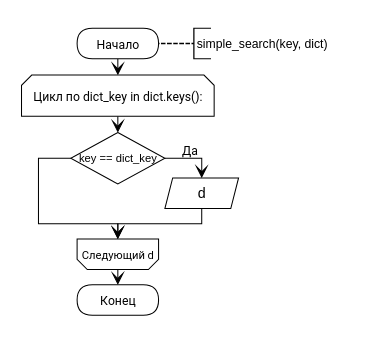
\includegraphics[scale=0.6]{full_search.jpg}
		\caption{Алгоритм полного перебора.}
		\label{fig:full}
	\end{center}
\end{figure}

\begin{figure}[h]
	\begin{center}
		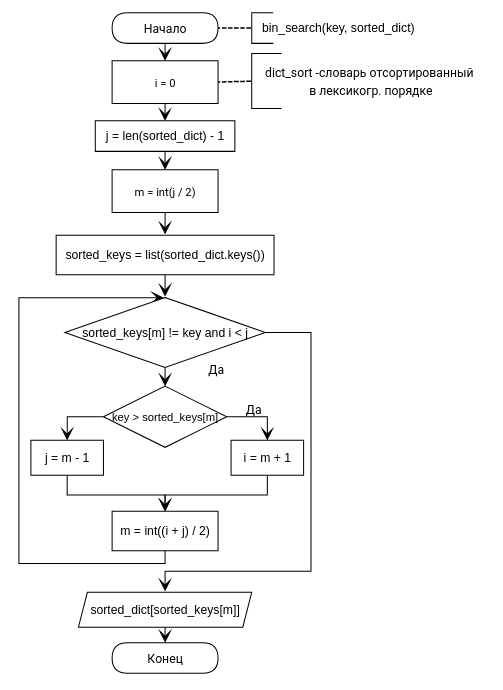
\includegraphics[scale=0.9]{bin_search.png}
		\caption{Алгоритм бинарного поиска.}
		\label{fig:bin}
	\end{center}
\end{figure}

\begin{figure}[h]
	\begin{center}
		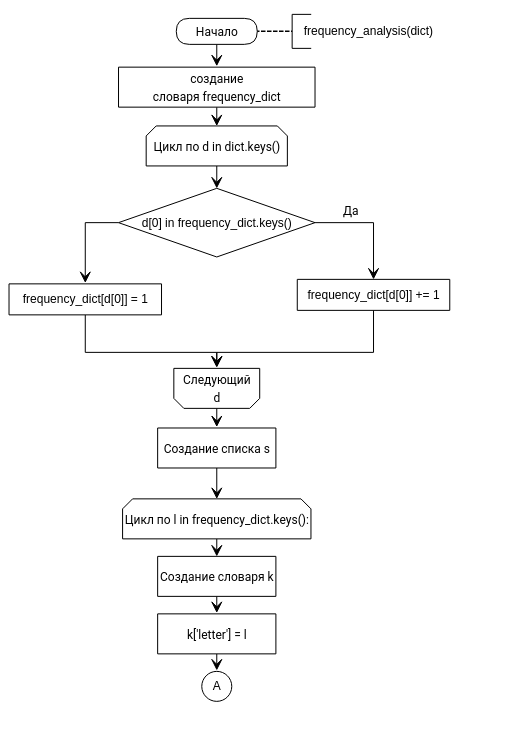
\includegraphics[scale=0.9]{freq1.png}
		\caption{Алгоритм частотного анализа, часть 1.}
		\label{fig:freq1}
	\end{center}
\end{figure}

\begin{figure}[h]
	\begin{center}
		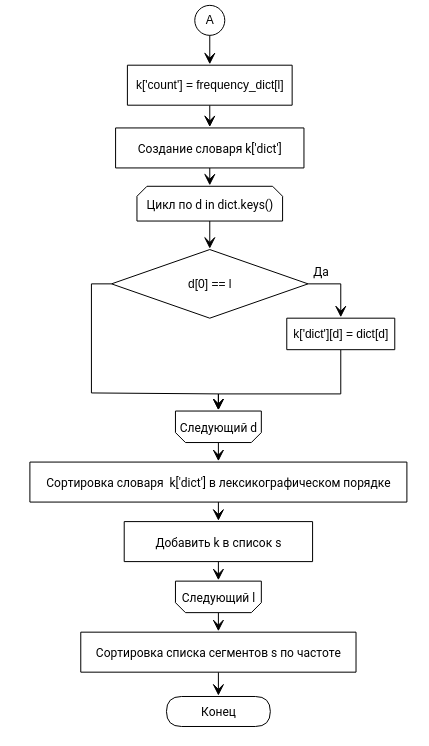
\includegraphics[scale=0.8]{freq2.png}
		\caption{Алгоритм частотного анализа, часть 2.}
		\label{fig:freq2}
	\end{center}
\end{figure}

\begin{figure}[h]
	\begin{center}
		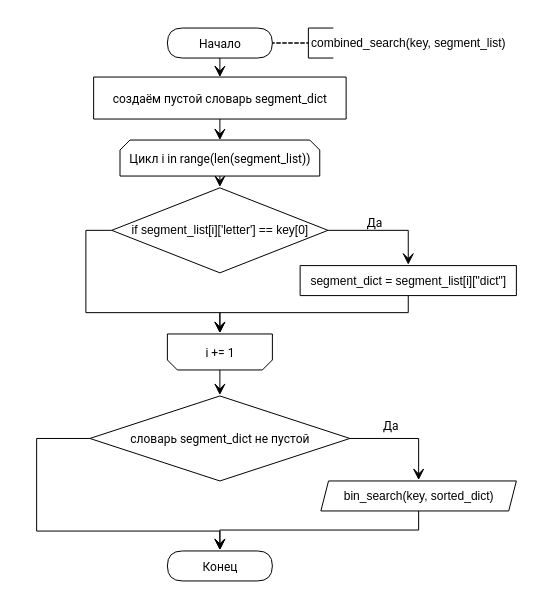
\includegraphics[scale=0.9]{combine.png}
		\caption{Комбинированный алгоритм.}
		\label{fig:combi}
	\end{center}
\end{figure}

\clearpage
\newpage

\section{Требования к программному обеспечению}

\begin{enumerate}
	\item В словаре должно быть более 1000 вхождений.
	
	\item Словарь является уникальным в пределах потока.
	
\end{enumerate}


\section{Вывод}
	В данном разделе представлено описание требований и допущений к программе и схемы алгоритмов.

\chapter{Технологическая часть}
В этом разделе будет обоснован выбор языка програмирования и будут приведены листинги кода реализованных алгоритмов.

\section{Выбор ЯП}
В качестве языка программирования мной был выбран Python, так как этот язык удобен для работы с файлами и словарями.
Для замера времени выполнения использовалась функция $time()$ из библиотеки time.

\section{Реализация алгоритмов}

В листингах 3.1 - 3.4 представлена реализация алгоритмов.

\begin{lstlisting}[label={lst:1},caption= Алгоритм полного перебора.]
	def search_simple(key, dict):
	for dict_key in dict.keys():
	if key == dict_key:
	return dict[key]
	return None
\end{lstlisting}

\begin{lstlisting}[label={lst:conv1},caption=Алгоритм бинарного поиска.]
	def bin_search(key, sorted_dict):
	sorted_keys = list(sorted_dict.keys())
	i = 0
	j = len(sorted_dict) - 1
	m = int(j / 2)
	while sorted_keys[m] != key and i < j:
	if key > sorted_keys[m]:
	i = m + 1
	else:
	j = m - 1
	m = int((i + j) / 2)
	if i > j:
	return None
	else:
	return sorted_dict[sorted_keys[m]]
\end{lstlisting}


\begin{lstlisting}[label={lst:conv1},caption=Частотный анализ.]
	def frequency_analysis(dict):
	frequency_dict = {}
	for d in dict.keys():
	if d[0] in frequency_dict.keys():
	frequency_dict[d[0]] += 1
	else:
	frequency_dict[d[0]] = 1
	
	s = []
	for l in frequency_dict.keys():
	k = {}
	k['letter'] = l
	k['count'] = frequency_dict[l]
	k['dict'] = {}
	for d in dict.keys():
	if d[0] == l:
	k['dict'][d] = dict[d]
	
	sorted_list = sorted(k['dict'].items())
	sorted_dict = {}
	for i in range(len(sorted_list)):
	sorted_dict[sorted_list[i][0]] = sorted_list[i][1]
	k['dict'] = sorted_dict
	
	s.append(k)
	
	
	s.sort(key=lambda val: val['count'], reverse=True)
	return s
\end{lstlisting}

\begin{lstlisting}[label={lst:conv1},caption=Комбинированный алгоритм.]
	def combined_search(key, segment_list):
	
	segment_dict = {}
	for i in range(len(segment_list)):
	if segment_list[i]['letter'] == key[0]:
	segment_dict = segment_list[i]["dict"]
	
	if len(segment_dict) == 0:
	return None
	
	return bin_search(key, sorted_dict)
	
\end{lstlisting}

\newpage

\section{Тестовые данные}

В таблице \ref{tab:tests} представлено тестирование программы.
\newline Тест 1 - ключ отсутсвует в словаре.
\newline Тест 2 - ключ является первым элементом словаря.
\newline Тест 3 - ключ является последним элементом словаря.
\newline Тест 4 - ключ является произвольным элементом словаря.

\begin{table}[h]
	\caption{\label{tab:tests}Функциональные тесты}
	\begin{center}
		\begin{tabular}{ | c | c | c | c |}
			\hline
			\textbf{Ключ} & \textbf{Перебор} & \textbf{Бинарный поиск} & \textbf{Комбинированный}\\ \hline
			'2000' &
			Ключ не найден & 
			Ключ не найден! &
			Ключ не найден \\
			\hline
			
			'1' & 
			{'sad'} &
			{'sad'} &
			{'sad'}  \\
			\hline
			
			'1500' &
			{'pa'} &
			{'pa'} &
			{'pa'} \\
			\hline
			
			'23' &
			{'je'} &
			{'je'} &
			{'je'} \\
			\hline
		\end{tabular}
		
	\end{center}
\end{table} 


Фактические результаты тестов совпали с ожидаемыми результатами.

\section{Вывод}
В этом разделе обоснован выбор языка програмирования, описаны технические характеристики,приведены листинги кода реализованных алгоритмов. Программа прошла тестирование и работает правильно.


\chapter{Исследовательская часть}

В этом разделе будет приведена демонстрация работы программы и будет исследование полученных результатов.

\section{Пример работы}

Демонстрация работы программы приведена на рисунках \ref{fig:prog_show1}, \ref{fig:prog_show2}. На вход подаётся ключ для поиска в словаре.

\begin{figure}[h]
	\begin{center}
		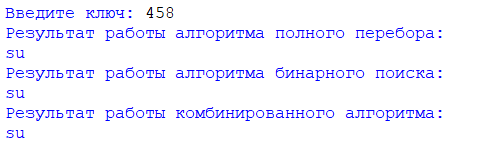
\includegraphics[scale=0.8]{prim1.png}
		\caption{Введённый ключ существует.}
		\label{fig:prog_show1}
	\end{center}
\end{figure}

\begin{figure}[h]
	\begin{center}
		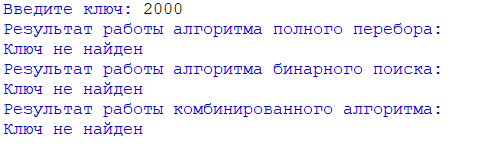
\includegraphics[scale=0.8]{prim2.png}
		\caption{Введённый ключ не существует.}
		\label{fig:prog_show2}
	\end{center}
\end{figure}

\section{Сравнение времени работы}
На рисунке \ref{fig:time1} представлено сравнение времени работы алгоритмов поиска по словарю перебором, бинарным поиском и комбинированным алгоритмом в лучшем, худшем,случайном случаях и при отсутствии ключа. Для каждого алгоритма представлено максимальное, минимальное и среднее время выполнения. Для замера времени каждая операция выполнялась 100 раз, среднее время выполнения взято как результат.

\begin{figure}[h]
	\begin{center}
		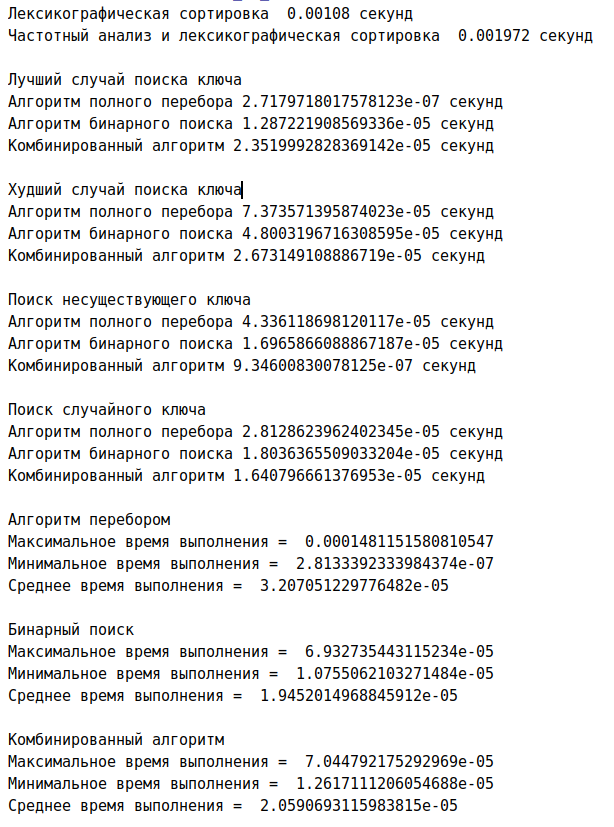
\includegraphics[scale=0.5]{time1.png}
		\caption{Время работы алгоритмов в разных случаях}
		\label{fig:time1}
	\end{center}
\end{figure}

Для алгоритма поиска перебором лучший случай - это поиск слов, которые находятся первыми в словаре, худший случай - поиск последних слов словаря.

Для алгоритма с бинарным поиском лучший случай - это поиск слова, которое находится в середине отсортированного в лексиграфическом порядке словаря, худший случай - слово находится при последнем делении диапазона поиска пополам.

Для комбинированного алгоритма лучший случай - это поиск слова, которое начинается на букву, которая чаще всего встречается в качестве первой буквы слова и находится в середине отсортированного в лексиграфическом порядке массива слов, начинающихся с этой же буквы; худший случай - слово, которое начинается на букву, которая реже всего встречается в качестве первой буквы слова и  находится при последнем делении диапазона поиска пополам (в этом случае время выбора нужного сегмента будет больше, но время поиска в этом коротком сегменте меньше).

На рисунке \ref{fig:time3} представлен график зависимости времени поиска от индекса ключа словаря, для построения которого использовались данные о времени поиска каждого элемента в словаре(1751 элемент). Индекс ключа указан на горизонтальной оси.

\begin{figure}[h]
	\begin{center}
		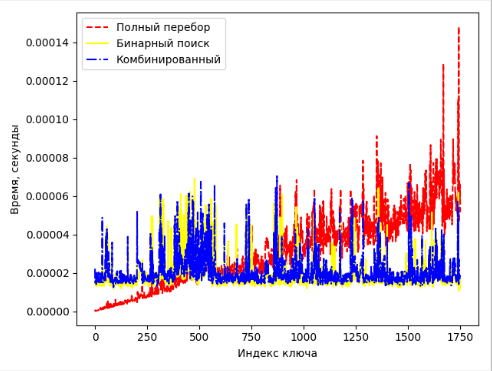
\includegraphics[scale=0.6]{time3.png}
		\caption{Время работы алгоритмов для поиска каждого ключа словаря}
		\label{fig:time3}
	\end{center}
\end{figure}

\newpage
 Для большей наглядности будем использовать для постоения графика меньше точек(возьмём данные о времени поиска каждого пятнадцатого элемента словаря). График зависимости времени поиска от индекса ключа словаря представлен на рисунке \ref{fig:time2}.

\begin{figure}[h]
	\begin{center}
		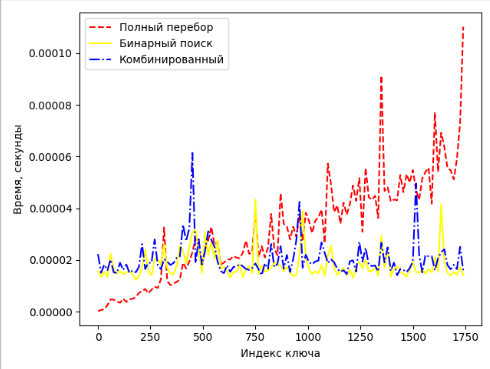
\includegraphics[scale=0.55]{time2.png}
		\caption{Время работы алгоритмов для поиска каждого пятнадцатого ключа словаря}
		\label{fig:time2}
	\end{center}
\end{figure}

\clearpage
\newpage

\section{Гистограммы}

\begin{figure}[h]
	\begin{center}
		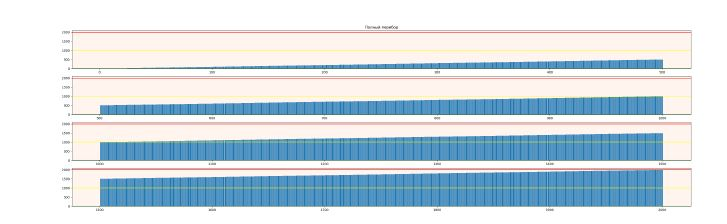
\includegraphics[scale=1]{gist1.jpg}
		\caption{Полный перебор, гистограмма типа 1}
		\label{fig:full}
	\end{center}
\end{figure}

\begin{figure}[h]
	\begin{center}
		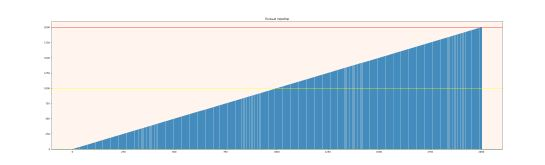
\includegraphics[scale=1]{gist2.jpg}
		\caption{Полный перебор, гистограмма типа 2}
		\label{fig:full}
	\end{center}
\end{figure}

\begin{figure}[h]
	\begin{center}
		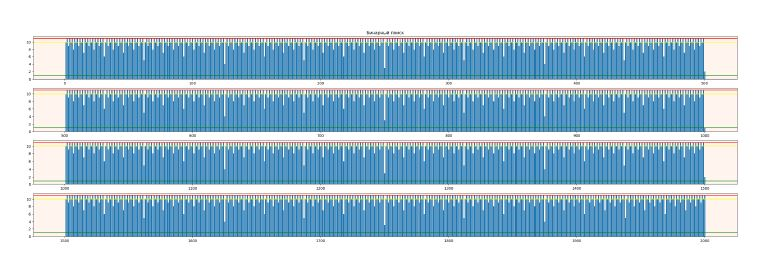
\includegraphics[scale=1]{gist3.jpg}
		\caption{Бинарный поиск, гистограмма типа 1}
		\label{fig:full}
	\end{center}
\end{figure}

\begin{figure}[h]
	\begin{center}
		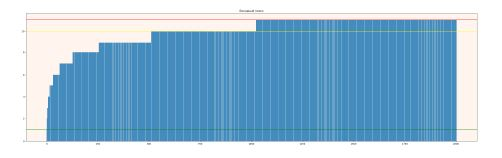
\includegraphics[scale=0.6]{gist4.jpg}
		\caption{Бинарный поиск, гистограмма типа 2}
		\label{fig:full}
	\end{center}
\end{figure}

\begin{figure}[h]
	\begin{center}
		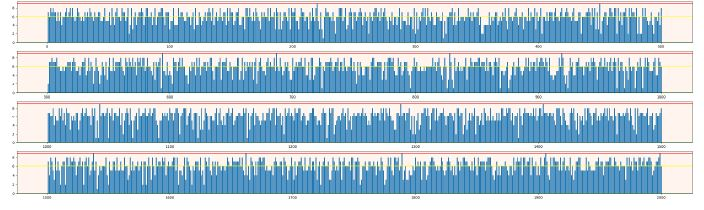
\includegraphics[scale=1]{gist5.jpg}
		\caption{Комбинированный алгоритм, гистограмма типа 1}
		\label{fig:full}
	\end{center}
\end{figure}

\begin{figure}[h]
	\begin{center}
		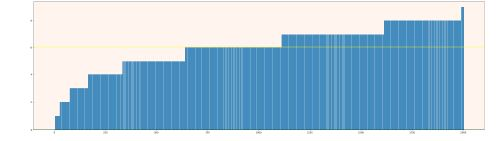
\includegraphics[scale=1]{gist6.jpg}
		\caption{Комбинированный алгоритм, гистограмма типа 2}
		\label{fig:full}
	\end{center}
\end{figure}

\clearpage
\newpage

\section{Вывод}

Как видно из графиков на рисунках \ref{fig:time3}, \ref{fig:time2} самый медленный алгоритм - алгоритм полного перебора. Время в нём растет линейно и увеличивается с увеличением индекса элемента словаря. Алгоритм бинарного поиска и комбинированный алгоритм трятят примерно одинаковое количество времени, при этом они требуют дополнительных расходов времени на подготовку данных к работе с алгоритмом, но эти расходы малы.

Однако в лучшем случае алгоритм перебором показывает самые лучшие результаты. Он работает в 4 раза быстрее алгоритма бинарного поиска и в 8 раз быстрее комбинированного алгоритма.

В худшем случае алгоритм перебором затрачивает в 1.75 раза больше времени, чем бинарный поиск и в 3.5 раза больше времени чем комбинированный алгоритм. Комбинированный алгоритм в худшем случае работает быстрее остальных алгоритмов. При поиске несуществующего ключа комбинированный алгоритм тоже работает быстрее всех.


\chapter*{Заключение}
\addcontentsline{toc}{chapter}{Заключение}

В ходе данной лабораторной работы была достигнута цель: изучены и реализованы алгоритмы поиска по словарю.

Для достижения поставленной цели выполнены следующие задачи.
\begin{enumerate}
	\item Реализован алгоритм поиска по словарю с использованием полного перебора, двоичного поиска, комбинированного алгоритма.
	
	\item Изучен алгоритм частотного анализа в задаче поиска по словарю;
	
	\item Проведено тестирование работы алгоритмов в худшем, лучшем и произвольном случаях.
	
	\item Проведены замеры процессорного времени работы алгоритмов поиска по словарю для каждого ключа и для отсутствующего ключа, вывести минимальное, максимальное и среднее время поиска ключа.
	
	\item Сделаны выводы на основе произведённого исследования.

\end{enumerate}

Алгоритм полного перебора работает хорошо в лучшем случае (когда искомые ключи находятся в самом начале словаря). Однако для работы лучше использовать алгоритм бинарного поиска или комбинированный алгоритм. Они работают примерно одинаково по времени, но комбинированный алгоритм выигрывает в случае несуществующего ключа или худшем случае. В среднем алгоритм полного перебора работает в два раза дольше чем остальные алгоритмы.

\addcontentsline{toc}{chapter}{Список литератури}

\bibliographystyle{utf8gost705u}  % стилевой файл для оформления по ГОСТу

\bibliography{51-biblio}          % имя библиографической базы (bib-файла)

\begin{thebibliography}{9}
	\addcontentsline{toc}{section}{Литература}
	\bibitem{foks} Словари (ассоциативные массивы) в Python [Электронный ресурс]. - Режим доступа: https://foxford.ru/wiki/informatika/slovari-assotsiativnye-massivy-v-python Дата обращения 30.11.2020.
	
	\bibitem{full} Алгоритмы последовательного поиска [Электронный ресурс]. - Режим доступа: https://cyberpedia.su/9x4e62.html Дата обращения 30.11.2020
	
	\bibitem{bin}Бинарный поиск [Электронный ресурс]. Режим доступа: https://prog-cpp.ru/search-binary/ Дата обращения 30.11.2020
	
	\bibitem{combi} Алгоритмы программирования [Электронный ресурс]. - Режим доступа: https://otus.ru/nest/post/829/ Дата обращения 30.11.2020
	
	\bibitem{time} Модуль time в Python [Электронный ресурс]. - Режим доступа: https://pythonru.com/osnovy/modul-time-v-python Дата обращения 01.12.2020
	
\end{thebibliography}

\end{document}
